%% Track overview, datasets, and descriptive statistics (main text).

\subsection{Experimental Design and Protocol}
\label{sec:exp-protocol}

We structured the evaluation program into four complementary tracks, fully documented under \path{docs/experimentos/} and \path{backend/experiments/results/}.

\textbf{Track~A --- Operational pipeline (24~months, Jul/2024--Jun/2026).} Continuous ingestion of NASA FIRMS CSVs, Open-Meteo weather, Nominatim geocoding, LangGraph orchestration (10~nodes), ReAct diagnostics, and RAG queries. Metrics: time-to-first-response, geocoding rate, agent success rate, backend availability, and inter-day FIRMS variability (e.g., 426\% day-over-day change on 2024-06-05 vs.\ 2024-06-06, validating the need for autonomous polling).

\textbf{Track~B --- Municipal fire prediction (Exp-B, v1--v9).} Iterative benchmark on synthetic then real data (Mar--Jun/2026): (v1--v2) next-day regression on simulated Ceará dynamics; (v3--v4) real FIRMS/INPE/Open-Meteo regression; (v5--v7) rare-event binary detection with Average Precision, persistence priors, and precision modes; (v8--v9) three-class alert system (NO/UNCERTAIN/YES). Temporal split 70/10/20\% (67/10/20~days). Models: MLP, LSTM, XGBoost, Koopman-Det, NeKo-PIGNN. Intermediate iteration tables (v1, v4--v7) are in \ref{app:exp-b}.

\textbf{Track~C --- GOES-16 unsupervised benchmark.} Validation against INPE BDQueimadas on 2024-10-31 (channels 7, 13, 14; hours 16--18~UTC; $72\times72$ grid). Methods: digital twin assimilation, isolation forest, spatial residual, \emph{combined persistence} (Lines~B in \path{docs/METODOLOGIA_NOVA_PROPOSTA.md}), and \emph{consensus ensemble} (Line~E, 2-of-3 vote). Reproducible via \path{src/unsupervised_fire_goes.py}; event-centered evaluation via \path{src/pixel_inpe_eval.py}.

\textbf{Track~D --- Agent, RAG, and risk-index calibration.} 100 operational ReAct questions; 30 RAG architecture queries (FAISS recall@5, manual completeness); heuristic risk classifier calibrated on 111{,}054 INPE records (\path{docs/calibracao/}).

\subsection{Reference Datasets and Descriptive Statistics}
\label{sec:hotspot-stats}

Table~\ref{tab:inpe-stats} summarizes INPE BDQueimadas records for Cear\'{a} (Jan/2024--Jun/2026): 111{,}639 records across 184 municipalities (99.5\% of the state) in the released dataset (\path{data/inpe_focos_ce/}); risk-calibration experiments (Section~\ref{sec:risk-calibration-exp}) used a 111{,}054-record snapshot taken on 12/Jun/2026, before the final records for May--June 2026 were appended. The dry season (Jul--Dec) concentrates approximately 93\% of annual activity in both complete years. Note that 2025 records exceed 2024 by more than an order of magnitude (94{,}135 vs.\ 7{,}160): 2025 combined an extreme dry season with the multi-satellite BDQueimadas export (NOAA-20/21, NPP, AQUA, GOES-19), whereas the 2024 export in the released dataset lacks per-satellite attribution and likely undercounts total detections; year-over-year comparisons should therefore be interpreted with caution.

Figure~\ref{fig:evolucao-combined} shows monthly and daily temporal patterns used for alert calibration. The pronounced dry-season peaks justify season-aware thresholding in the three-class alert system (Section~\ref{sec:three-level}).

\begin{resulttable}{INPE hotspot descriptive statistics for Cear\'{a}, computed from the released dataset (Jan/2024--Jun/2026; 111{,}639 records).}{tab:inpe-stats}
\begin{tabular}{@{}lrrr@{}}
\toprule
\textbf{Metric} & \textbf{2024} & \textbf{2025} & \textbf{2026 (Jan--Jun)} \\
\midrule
Total hotspots & 7{,}160 & 94{,}135 & 10{,}344 \\
Mean monthly (dry season) & 1{,}119 & 14{,}563 & --- \\
Mean monthly (rainy season) & 73 & 1{,}125 & 1{,}724 \\
Affected municipalities (monthly mean) & 68 & 138 & 97 \\
Peak daily count & 464 & 1{,}831 & 854 \\
Days with fire ($>0$ hotspots) & 198 & 359 & 157 \\
\bottomrule
\end{tabular}
\end{resulttable}

\begin{figure}[!htbp]
\centering
\begin{subfigure}[b]{0.48\linewidth}
  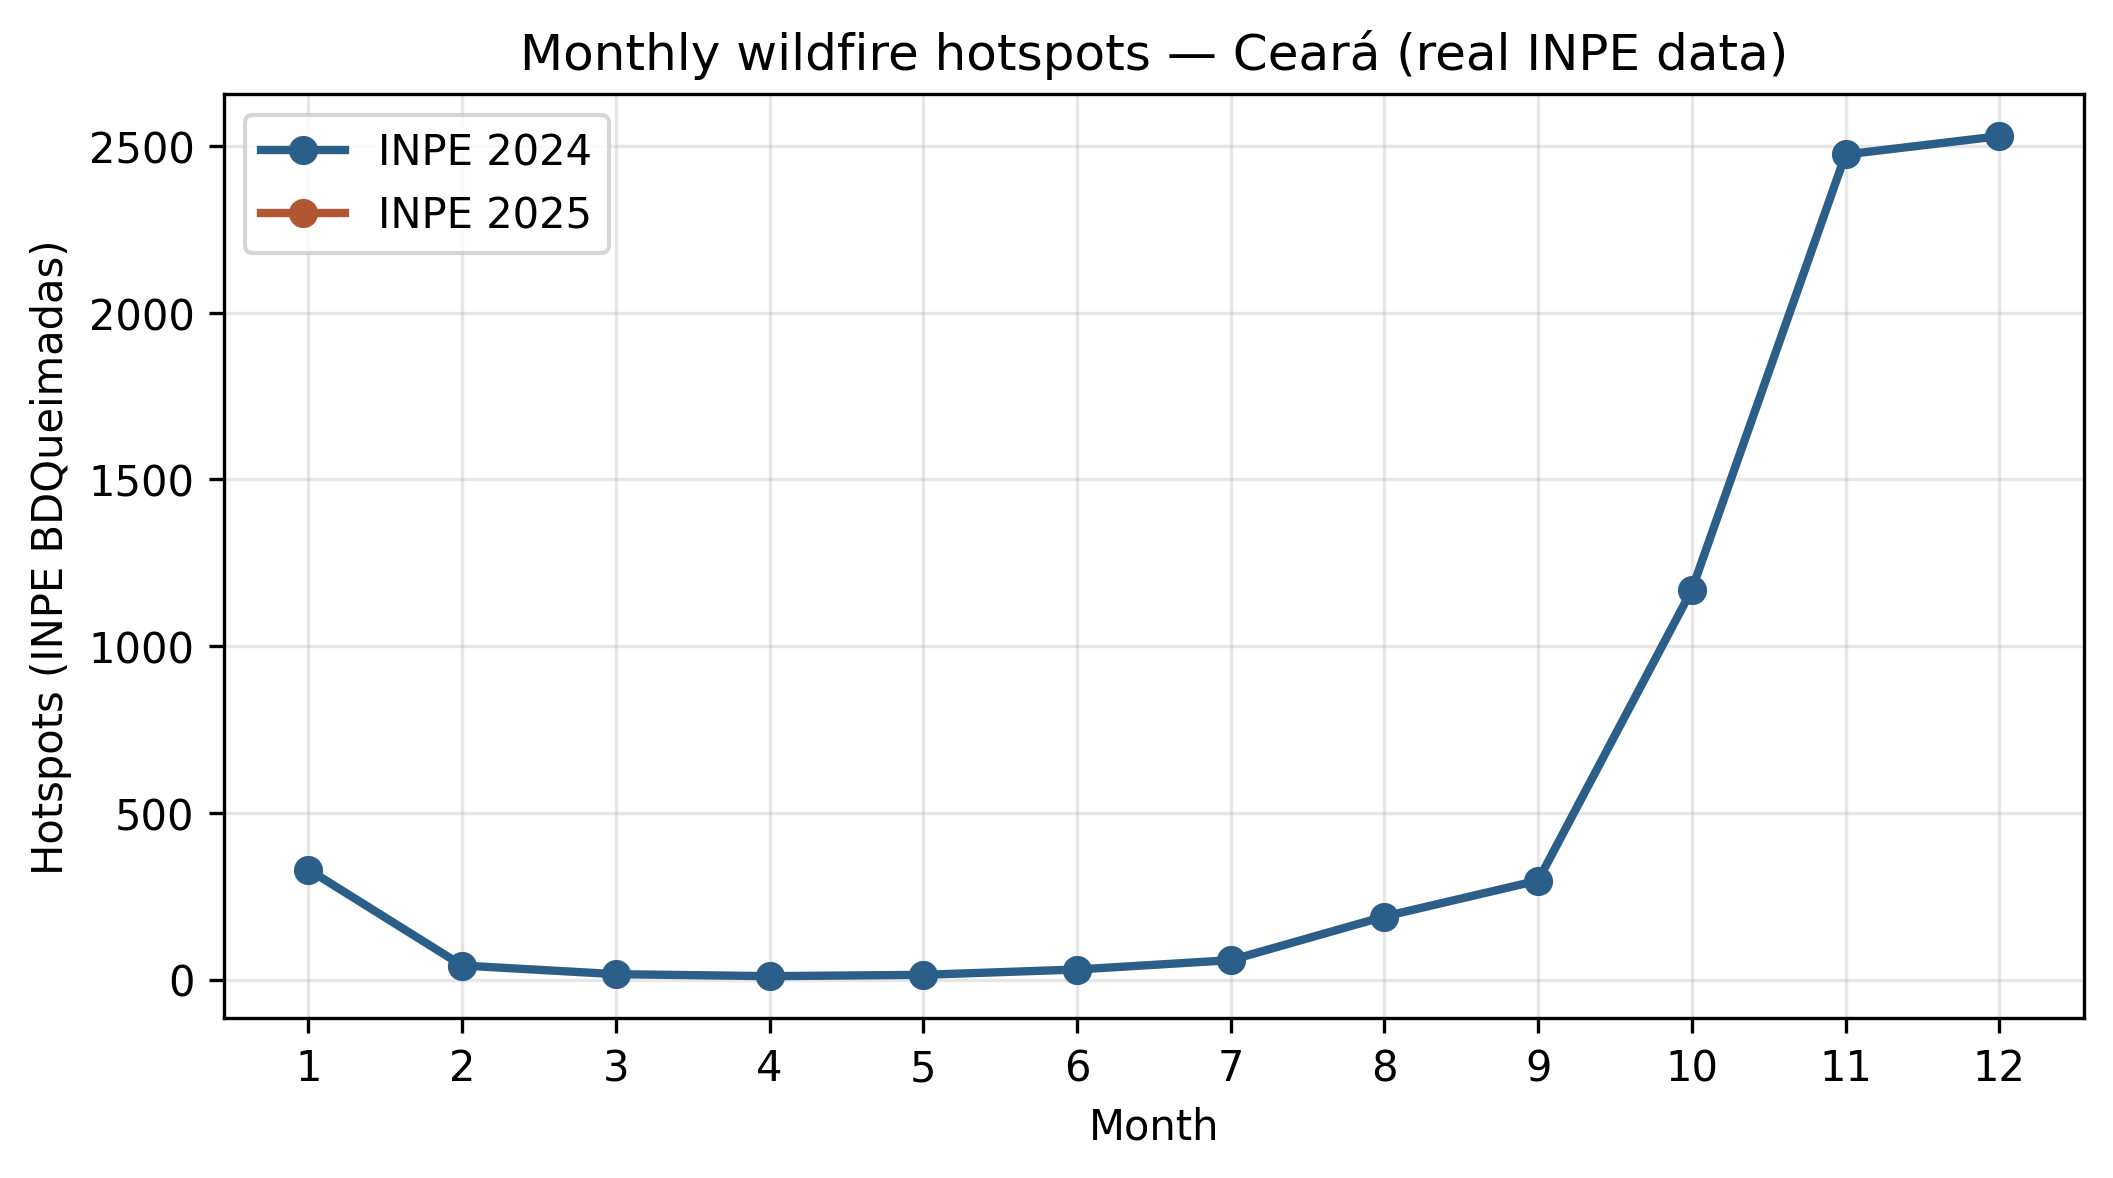
\includegraphics[width=\linewidth]{figures/evolucao-focos-inpe-real.png}
  \caption{Monthly evolution}
\end{subfigure}\hfill
\begin{subfigure}[b]{0.48\linewidth}
  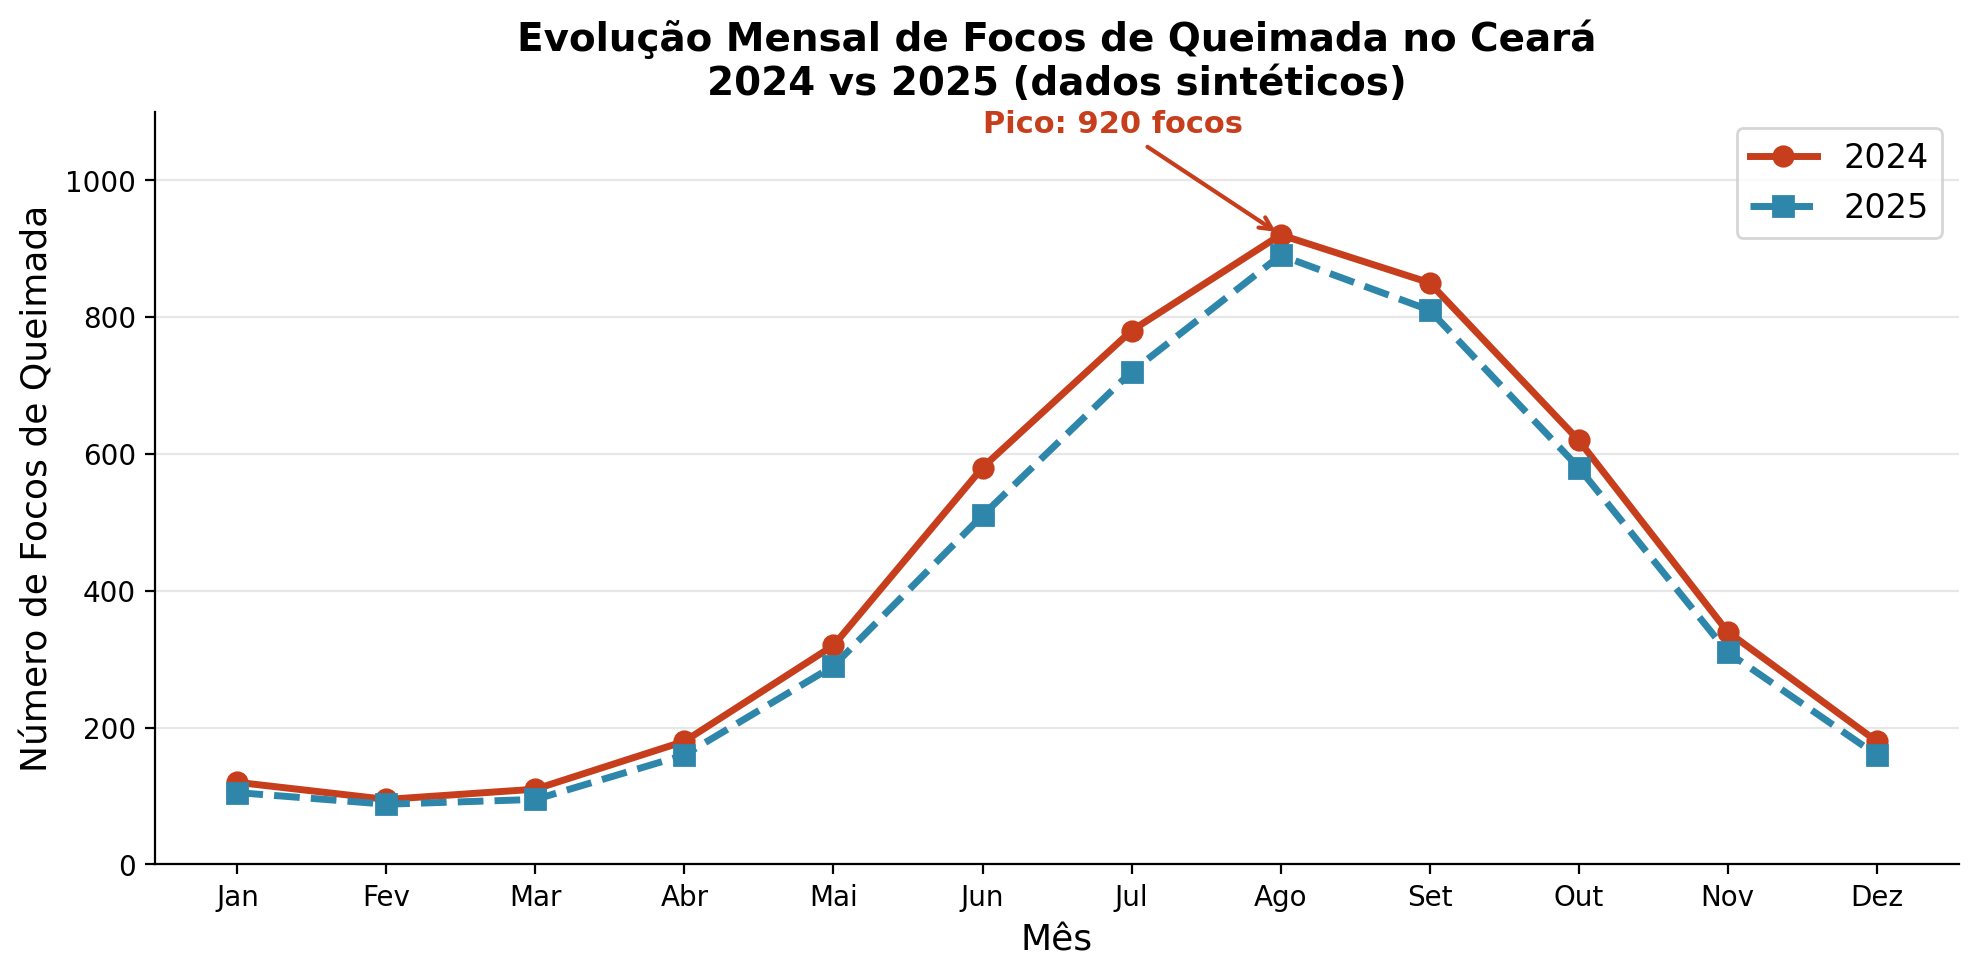
\includegraphics[width=\linewidth]{figures/evolucao-focos.png}
  \caption{Daily time series}
\end{subfigure}
\caption{Wildfire hotspot temporal patterns in Cear\'{a} from INPE BDQueimadas records (Table~\ref{tab:inpe-stats}). (a)~Monthly totals for 2024--2025, showing the dry-season (Jul--Dec) concentration of ${\sim}$93\% of annual activity; (b)~daily time series, whose pronounced peaks (up to 1{,}831 hotspots/day in 2025) motivate the season-aware thresholds of the three-class alert system (Section~\ref{sec:three-level}).}
\label{fig:evolucao-combined}
\end{figure}

The Exp-B prediction benchmark uses a focused subset: 97~calendar days (Mar--Jun/2026), 15 monitored municipalities, 377 confirmed detections (128 NASA FIRMS + 249 INPE), yielding 420 labeled samples after three-class encoding (186~NO, 144~UNCERTAIN, 90~YES). Split: 67~train / 10~validation / 20~test days (70/10/20\%). Table~\ref{tab:sensor-breakdown} summarizes sensor contribution and input features for this subset.

Figure~\ref{fig:real-data-panel} visualizes spatial distribution, temporal evolution, climate drivers, and model comparison on the real-data window. Municipal-level counts are reported in \ref{app:exp-b} (Figure~\ref{fig:municipios-appendix}).

\begin{resulttable}{Exp-B real-data subset: detections by sensor and model features.}{tab:sensor-breakdown}
\begin{minipage}[t]{0.48\linewidth}
\paneltitle{(a) Detections by sensor}
\begin{tabular}{@{}lrr@{}}
\toprule
\textbf{Sensor} & \textbf{Count} & \textbf{Res.} \\
\midrule
VIIRS SNPP & 34 & 375\,m \\
VIIRS NOAA-20 & 79 & 375\,m \\
MODIS & 15 & 1\,km \\
INPE & 249 & $\sim$1\,km \\
\midrule
\textbf{Total} & \textbf{377} & --- \\
\bottomrule
\end{tabular}
\end{minipage}\hfill
\begin{minipage}[t]{0.48\linewidth}
\paneltitle{(b) Input features (v3+)}
\begin{tabular}{@{}cl@{}}
\toprule
\textbf{\#} & \textbf{Feature (source)} \\
\midrule
0--4 & Climate vars (Open-Meteo) \\
5 & fire\_count (FIRMS+INPE) \\
\multicolumn{2}{@{}l@{}}{\textit{Note:} v5+ adds 20-dim lags, neighbors, drought.} \\
\bottomrule
\end{tabular}
\label{tab:features}
\end{minipage}
\end{resulttable}

\begin{figure}[!htbp]
\centering
\begin{subfigure}[b]{0.48\linewidth}
  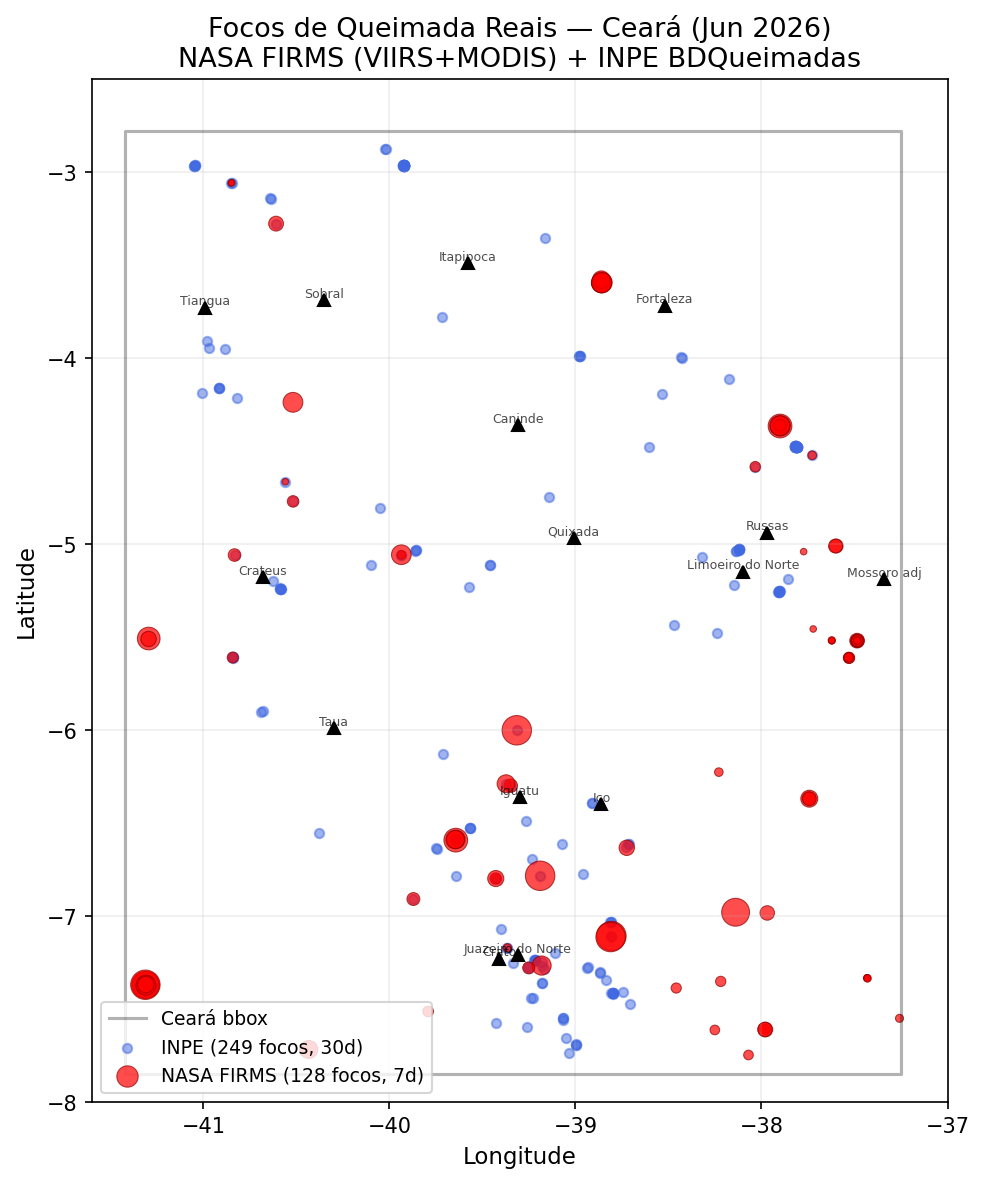
\includegraphics[width=\linewidth]{figures/experimentos/01_mapa_focos_reais.png}
  \caption{Spatial map}
\end{subfigure}\hfill
\begin{subfigure}[b]{0.48\linewidth}
  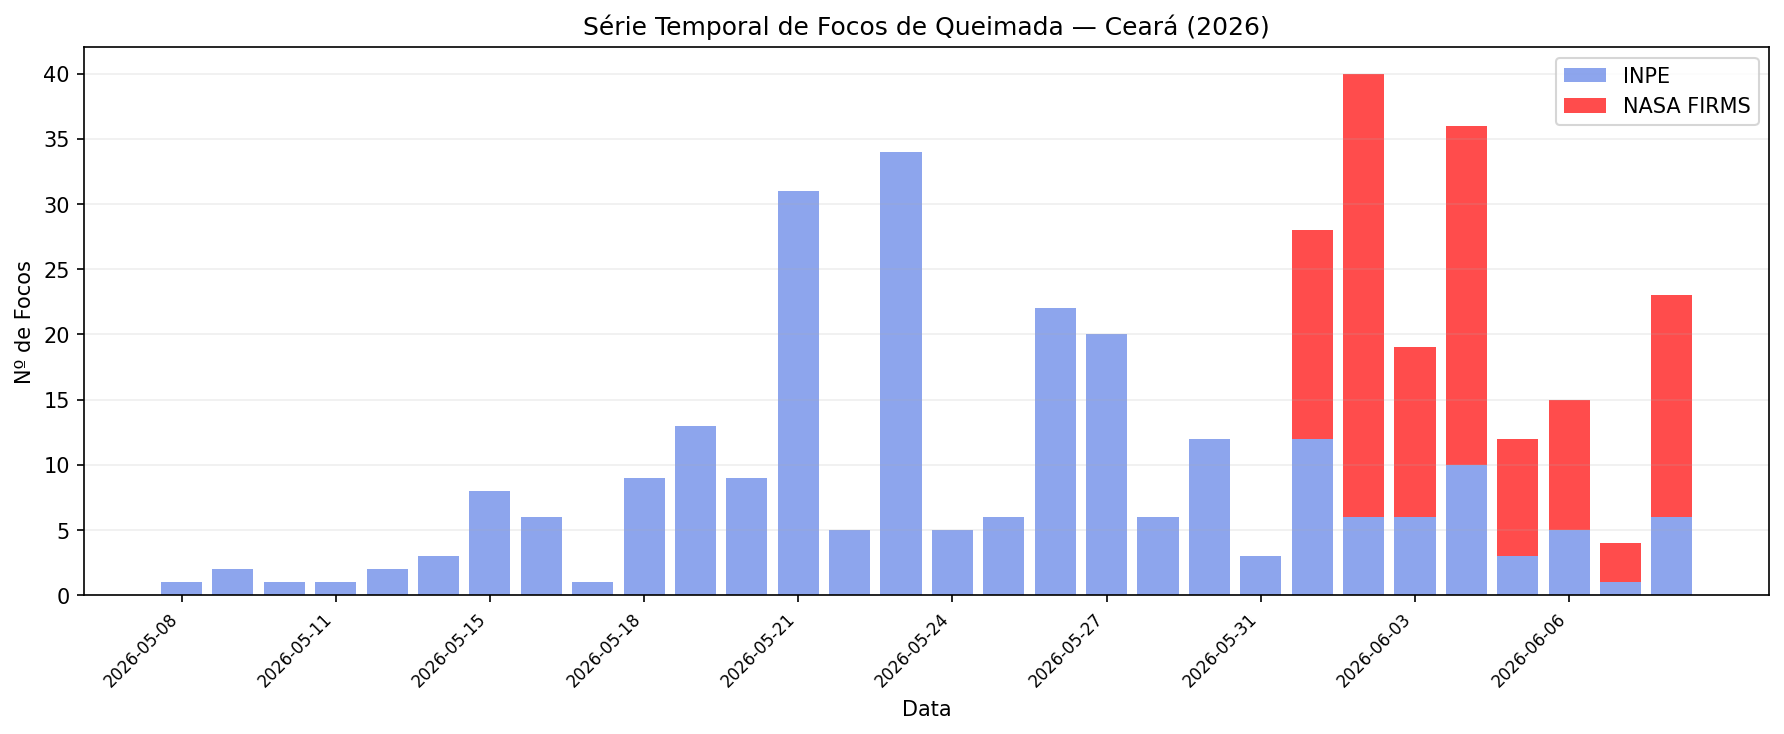
\includegraphics[width=\linewidth]{figures/experimentos/02_serie_temporal_focos.png}
  \caption{Daily series}
\end{subfigure}\\[0.4em]
\begin{subfigure}[b]{0.48\linewidth}
  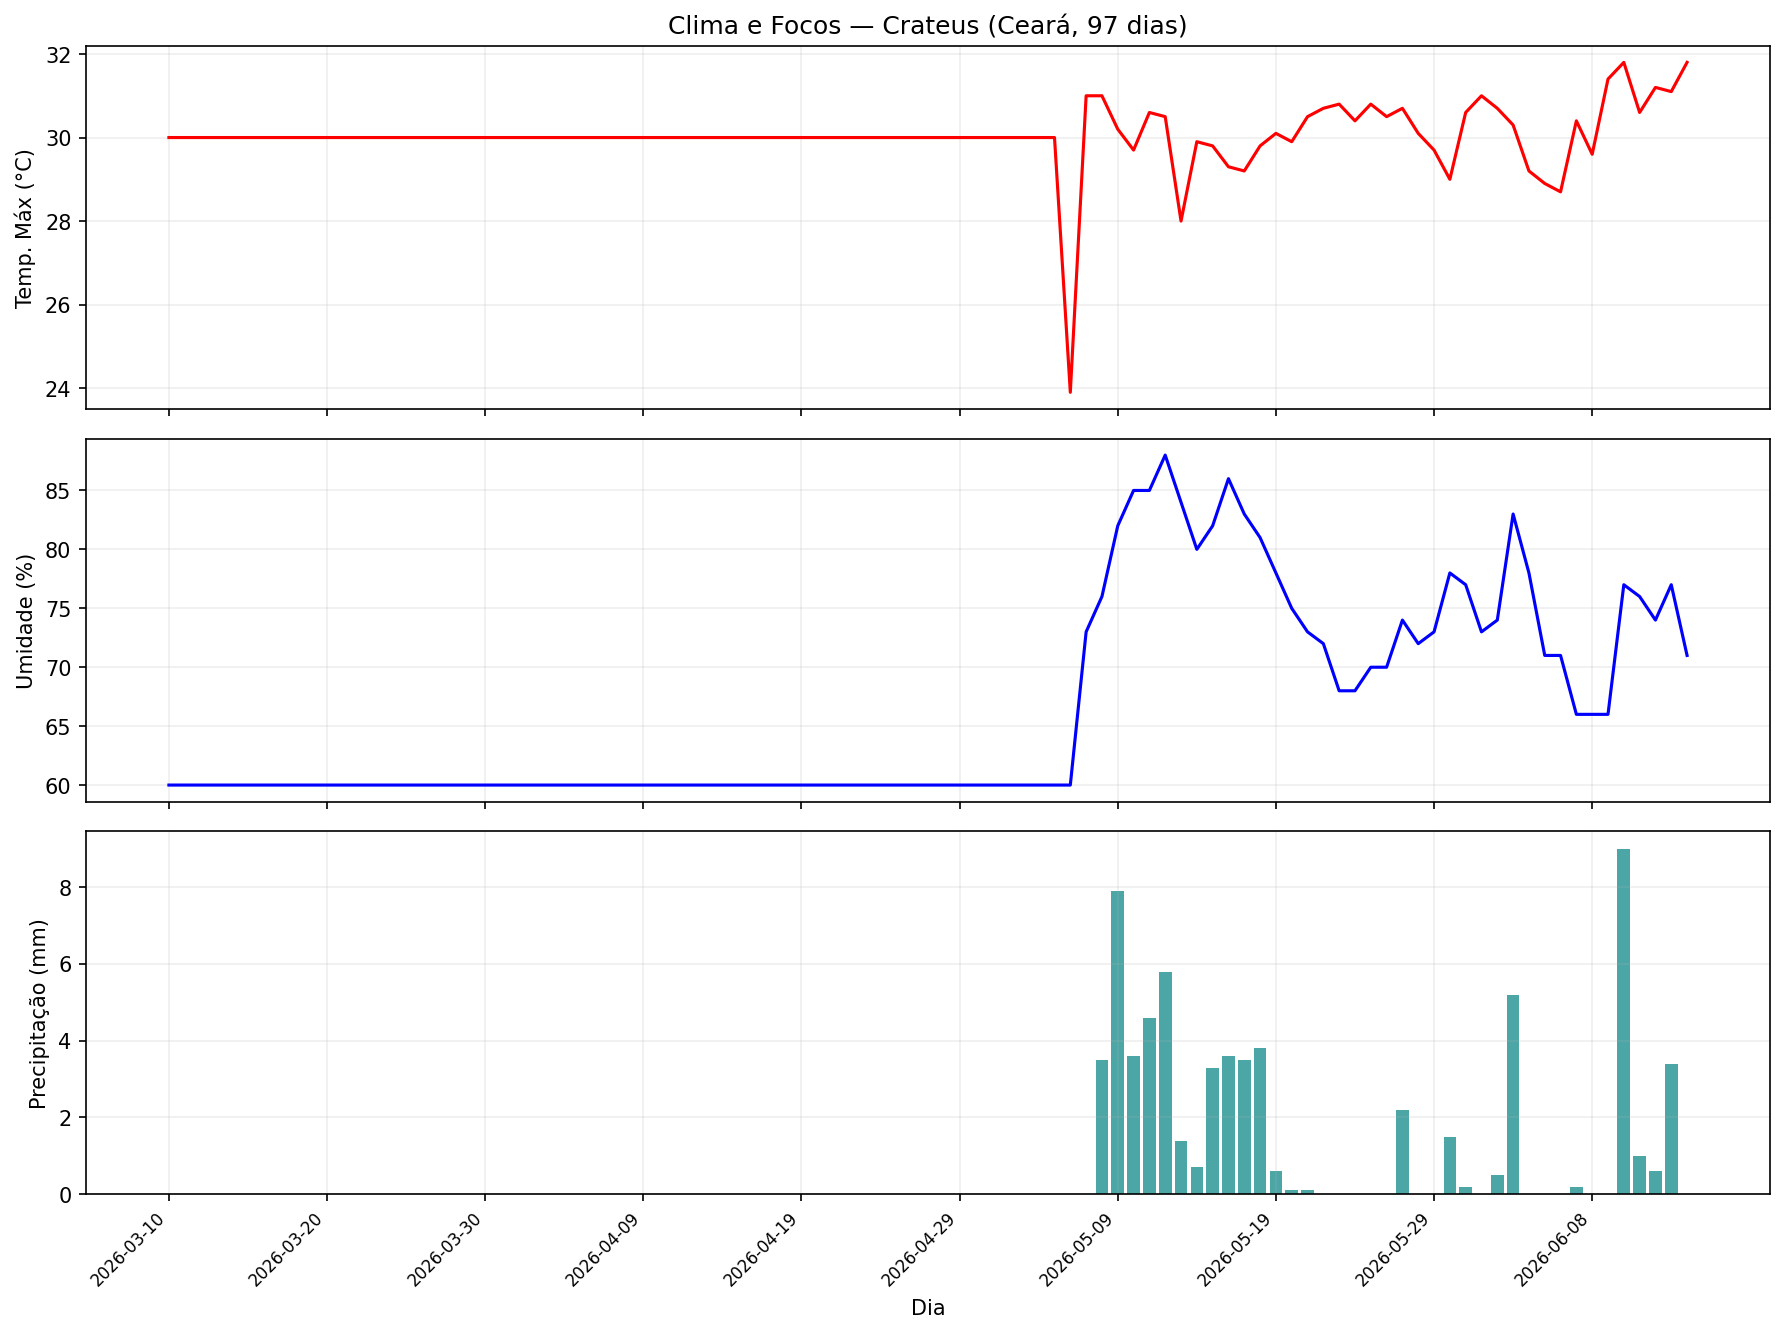
\includegraphics[width=\linewidth]{figures/experimentos/03_clima_crateus.png}
  \caption{Climate (Crate\'{u}s)}
\end{subfigure}\hfill
\begin{subfigure}[b]{0.48\linewidth}
  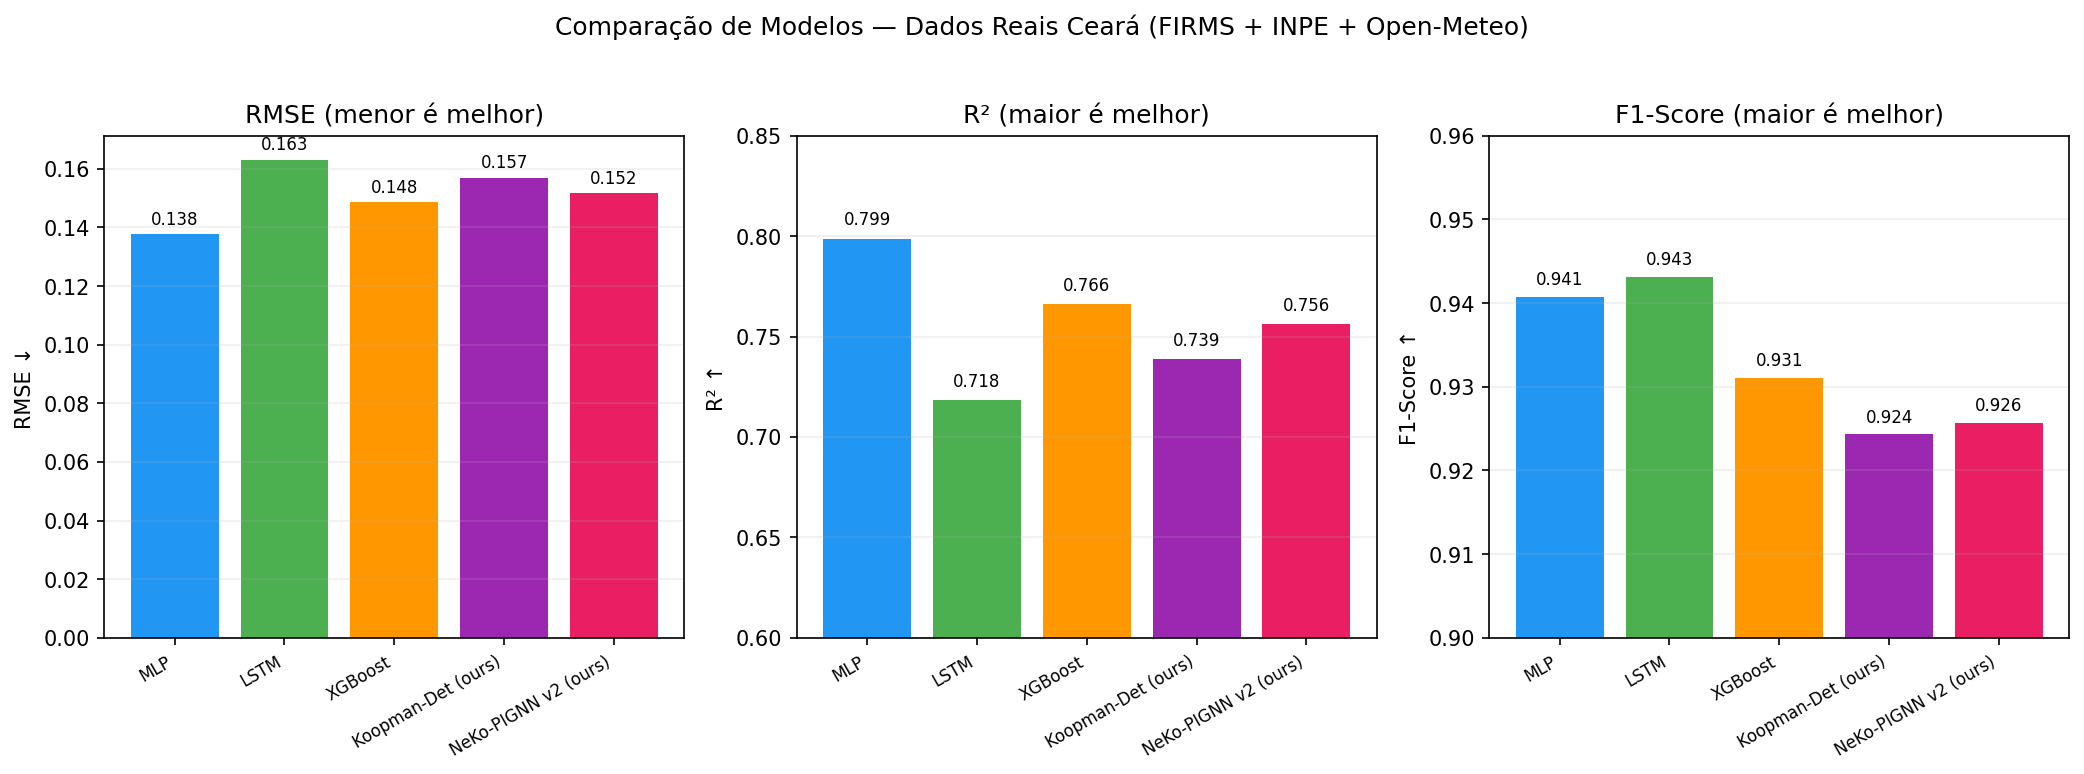
\includegraphics[width=\linewidth]{figures/experimentos/04_comparacao_modelos.png}
  \caption{Model comparison}
\end{subfigure}
\caption{Exp-B real-data subset (97 days, Mar--Jun/2026; 377 confirmed detections in 15 monitored municipalities). (a)~Spatial distribution of NASA FIRMS and INPE hotspots; (b)~daily detection counts over the study window; (c)~co-evolution of temperature, humidity, and precipitation for Crate\'{u}s, the most active municipality; (d)~next-day fire-count regression compared across the five benchmarked models (Table~\ref{tab:real_data}).}
\label{fig:real-data-panel}
\end{figure}
